\documentclass[10pt,a4paper]{article}
\usepackage{fullpage}
\usepackage{graphicx}
\usepackage{fancyhdr}
\usepackage{occi}
\setlength{\headheight}{13pt}
\pagestyle{fancy}

% default sans-serif
\renewcommand{\familydefault}{\sfdefault}

% no lines for headers and footers
\renewcommand{\headrulewidth}{0pt}
\renewcommand{\footrulewidth}{0pt}

% header
\fancyhf{}
\lhead{GWD-R}
\rhead{\today}

% footer
\lfoot{occi-wg@ogf.org}
\rfoot{\thepage}

% paragraphs need some space...
\setlength{\parindent}{0pt}
\setlength{\parskip}{1ex plus 0.5ex minus 0.2ex}

%\renewcommand\paragraph{%
%  \@startsection{paragraph}{4}{0mm}%
%     {-\baselineskip}%
%     {.5\baselineskip}%
%     {\normalfont\normalsize\bfseries}}

% some space between header and text...
\headsep 13pt

\setcounter{secnumdepth}{4}

\begin{document}

% header on first page is different
\thispagestyle{empty}

GWD-R \hfill  Thijs Metsch, Platform Computing\\
OCCI-WG \hfill  Andy Edmonds, Intel\\
\rightline {October 7, 2010}\\
\rightline {Updated: \today}

\vspace*{0.5in}

\begin{Large}
\textbf{Open Cloud Computing Interface - Infrastructure}
\end{Large}

\vspace*{0.5in}

\underline{Status of this Document}

This document provides information to the community regarding the
specification of the Open Cloud Computing Interface. Distribution is
unlimited.


\underline{Obsoletes}

This document obsoletes GFD-xxx [REFERENCE].

\underline{Copyright Notice}

Copyright \copyright Open Grid Forum (2009-2010). All Rights Reserved.

\underline{Trademarks}

OCCI is a trademark of the Open Grid Forum.

\underline{Abstract}

This document, part of a document series, produced by the OCCI working
group within the Open Grid Forum (OGF), provides a high-level
definition of a Protocol and API. The document is based upon
previously gathered requirements and focuses on the scope of important
capabilities required to support modern service offerings.


\newpage
\tableofcontents
\newpage

\section{Introduction}
The Open Cloud Computing Interface (OCCI) is a RESTful Protocol and
API for all kinds of management tasks. OCCI was originally initiated
to create a remote management API for IaaS%
\footnote{Infrastructure as a Service}
model-based services, allowing for the development of interoperable tools for
common tasks including deployment, autonomic scaling and monitoring.
%
It has since evolved into an flexible API with a strong focus on
interoperability while still offering a high degree of extensibility. The
current release of the Open Cloud Computing Interface is suitable to serve many
other models in addition to IaaS, including e.g.~PaaS and SaaS.

In order to be modular and extensible the current OCCI specification is
released as a suite of complimentary documents, which together form the complete
specification.
%
The documents are divided into three categories consisting of the OCCI Core,
the OCCI Renderings and the OCCI Extensions.
%
\begin{itemize}
\item The OCCI Core specification consists of a single document defining the
 OCCI Core Model. The OCCI Core Model can be interacted with {\em
 renderings} (including associated behaviours) and expanded through {\em extensions}.
\item The OCCI Rendering specifications consist of multiple documents each
 describing a particular rendering of the OCCI Core Model. Multiple renderings can
 interact with the same instance of the OCCI Core Model and will automatically support
 any additions to the model which follow the extension rules defined in OCCI
 Core.
\item The OCCI Extension specifications consist of multiple documents each
 describing a particular extension of the OCCI Core Model. The extension documents
 describe additions to the OCCI Core Model defined within the OCCI specification
 suite.
\end{itemize}
%
The current specification consist of three documents.
Future releases of OCCI may include additional rendering and extension
specifications. The documents of the current OCCI specification suite are:

\begin{description}
\item[OCCI Core] describes the formal definition of the the OCCI Core Model
\cite{occi:core}.
\item[OCCI HTTP Rendering] defines how to interact with the OCCI Core Model using the
RESTful OCCI API \cite{occi:http_rendering}. The document defines how the OCCI Core Model can
be communicated and thus serialised using the HTTP protocol.
\item[OCCI Infrastructure] contains the definition of the OCCI Infrastructure
extension for the IaaS domain \cite{occi:infrastructure}. The document defines
additional resource types, their attributes and the actions that can be taken
on each resource type.
\end{description}


OCCI makes an ideal interoperable boundary interface between the web and the
internal resource management system of infrastructure providers.

\section{Notational Conventions}
All these parts and the information within are mandatory for
implementors (unless otherwise specified). The key words "MUST", "MUST
NOT", "REQUIRED", "SHALL", "SHALL NOT", "SHOULD", "SHOULD NOT",
"RECOMMENDED", "MAY", and "OPTIONAL" in this document are to be
interpreted as described in RFC 2119 \cite{rfc2119}.

\textbf{Andy: we need to state that this document as part of the current document set,
supersedes all previous documents.}


UML activity diagrams do not specify how OCCI should be rendered but what
possible request and outcomes can be.

% begin infrastructure content

\section{Infrastructure}

The main infrastructure domain Resource types within OCCI, including their specification definitions, are:
\begin{itemize}
\item Compute: Information processing resources.
\item Network: Interconnection resources.
\item Storage: Information recording resources.
\end{itemize}
These infrastructure Resource types inherit the core Resource base type and all its attributes. OCCI implementors MUST implement these types. The HTTP Rendering document defines how to interact with these resource types using RESTful communication.

As REQUIRED by the OCCI Core specification every resource type instantiated that is a subclass of Resource MUST be assigned a Category that identifies the instantiated resource type. Each such Category MUST be related to the Resource base type Category. These Categories, the core categories, MUST always remain immutable to any client.

The following table describe the Category defined for each of the infrastructure Resource subtypes:

\mytablefloat{\label{tbl:kinds}The structural \hl{Kind} instances defined for
the infrastructure sub-types of \hl{Resource} and \hl{Link}}{
\begin{tabular}{llll}
Term & Scheme & Title & Related structural \hl{Kind} \\
\hline
compute & http://schemas.ogf.org/occi/infrastructure\# & Compute Resource & http://schemas.ogf.org/occi/core\#resource \\
storage & http://schemas.ogf.org/occi/infrastructure\# & Storage Resource & http://schemas.ogf.org/occi/core\#resource \\
network & http://schemas.ogf.org/occi/infrastructure\# & Network Resource & http://schemas.ogf.org/occi/core\#resource \\
\end{tabular}
}

The following sections on Compute, Storage and Network detail the Attributes and Actions defined for each resource type.

\subsection{Compute}
The Compute \hl{Resource} type represent a generic information processing
resource.
The Compute \hl{Resource} type is assigned the structural \hl{Kind}
\textit{http://schemas.ogf.org/occi/infrastructure\#compute}.
\marginpar{Only this section has been updated with the proper
wording as introduced in Core. Please perfect this section before converting
the other sections to the same style!}

\mytablefloat{\label{tbl:compute}Attributes defined for the Compute
\hl{Resource} type. The attributes are defined by the Compute \hl{Resource}
type's structural \hl{Kind}
\textit{http://schemas.ogf.org/occi/infrastructure\#compute}}{
\begin{tabular}{lp{2.5cm}p{1cm}lp{6cm}}
\toprule
Attribute&Type&Multi\-plicity&Mutability&Description\\
\colrule
occi.compute.architecture & Enum \{x86, x64\} & 1 & Mutable & CPU Architecture of the instance.\\
occi.compute.cores & Integer & 1 & Mutable & Number of CPU cores assigned to the instance.\\
occi.compute.hostname & String & 0\ldots1 & Mutable & Fully Qualified DNS hostname for the instance.\\
occi.compute.speed & Float, ${\mathbf 10}^9$ (GHz) & 1 & Mutable & CPU Clock frequency (speed) in gigahertz.\\
occi.compute.memory & Float, ${\mathbf 10}^9$ (GiB) & 1 & Mutable & Maximum RAM in gigabytes allocated to the instance.\\
occi.compute.state & Enum \{active, inactive, suspended\} & 1 & Immutable & Current state of the instance.\\
\botrule
\end{tabular}
}

Table~\ref{tbl:compute} describe the attributes defined for the Compute
\hl{Resource} type through its structural \hl{Kind}. These attributes MUST be
exposed by an instance of the Compute \hl{Resource} type.

\mytablefloat{\label{tbl:compute_actions}%
\hl{Action}s defined by the structural \hl{Kind}
\textit{http://schemas.ogf.org/occi/infrastructure\#compute}. Every \hl{Action}
in the table is identified by a \hl{Category} instance using the
\textit{http://schemas.ogf.org/occi/infrastructure/compute/action\#}
categorisation scheme. ``Action term'' below refer to the term of the \hl{Action}'s
\hl{Category} identifier}{
\begin{tabular}{lll}
\toprule
Action term & Target state & Parameters \\
\colrule
start & active & -- \\
stop & inactive & Enum \{graceful, acpioff, poweroff\} \\
restart & active (via stop and start chain) & Enum \{graceful, warm, cold\} \\
suspend & suspended & Enum \{hibernate, suspend\} \\
\botrule
\end{tabular}
}

Table~\ref{tbl:compute_actions} describe the \hl{Action}s defined for the
Compute \hl{Resource} type by its structural \hl{Kind}.
% FIXME - The structural Kind is indeed REQUIRED to expose all Actions defined
% but what is required from a Compute instance? Only applicable Actions?
%
% These \hl{Action}s MUST be exposed by an instance of the Compute \hl{Resource}
% type.
%
Figure~\ref{fig:compute_state} illustrate the state diagram for a Compute
\hl{Resource} instance.

\begin{figure}[!h]
	\centering
	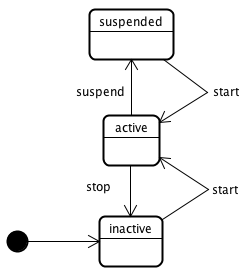
\includegraphics[scale=0.4]{figs/compute-state.png}
	\caption{State diagram for the Compute \hl{Resource} type}
	\label{fig:compute_state}
\end{figure}

\subsection{Network}
Network represents a L2 networking entity (e.g. a virtual switch). It can be extended using the mix-in mechanism or sub-classed to support L3/L4 capabilities such as TCP/IP etc. For the purposes of this specification we define a suitable OCCI mix-in so that IP networking can be supported. 

The Network Resource type is assigned the http://schemas.ogf.org/occi/infrastructure\#network Category. A Network Resource instance MUST use and expose this Category.

\subsubsection{Attributes}
The attributes that MUST be exposed by an instance of the Network Resource type are as follows:

\begin{tabular}{lllll}
Attribute&Type&Multiplicity&Mutability&Description\\
\hline
occi.network.vlan & Integer, 0-4095 & 0\ldots1 & Mutable & 802.1q VLAN Ientifier (e.g. 4095).\\
occi.network.label & Token & 0\ldots1 & Mutable & Tag based VLANs (e.g. external-dmz).\\
% occi.network.address & IPv4 or IPv6 Address range, CIDR notation & 0\ldots* & Mutable & Internet Protocol(IP) network address (e.g. 192.168.0.1/24, fc00::/7)\\
% occi.network.gateway & IPv4 or IPv6 Address & 0\ldots1 & Mutable & Internet Protocol(IP) network address (e.g. 192.168.0.1/24, fc00::/7)\\
% occi.network.allocation & String Enumeration, {auto, dhcp, manual} & 0\ldots1 & Mutable & Address mechanism: auto use the provider default policy dhcp use the dynamic host configuration protocol manual use user supplied static network configurations.\\
occi.network.state & Enumeration, {active, inactive} & 1 & Immutable & Current state of the instance.\\
\end{tabular}

\subsubsection{Actions}
Actions can be performed upon instances of the Network Resource type. The set that must be supported are as follows:

\begin{tabular}{lll}
Action&Target State&Parameters\\
\hline
http://schemas.ogf.org/occi/infrastructure/network/action\#up & active & None\\
http://schemas.ogf.org/occi/infrastructure/network/action\#down & inactive & None\\
\end{tabular}

\subsubsection{States}
Below illustrates the state diagram based on the actions defined above.

%\clearpage
\begin{figure}[!h]
	\centering
	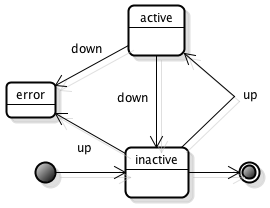
\includegraphics[scale=0.4]{figs/network-state.png}
	\caption{State diagram for Network}
	\label{fig:network_state}
\end{figure}

\subsubsection{IPNetworking Mixin}

In order to support L3/L4 capabilities (e.g. IP, TCP etc) an OCCI mixin is herewith defined. 

The IPNetworking mixin is assigned the http://schemas.ogf.org/occi/infrastructure/network\#ipnetwork Category. A IPNetworking mixin MUST use and expose this Category.

\begin{tabular}{lllll}
Attribute&Type&Multiplicity&Mutability&Description\\
\hline
occi. ipnetwork.address & IPv4 or IPv6 Address range, CIDR notation & 0\ldots* & Mutable & Internet Protocol(IP) network address (e.g. 192.168.0.1/24, fc00::/7)\\
occi. ipnetwork.gateway & IPv4 or IPv6 Address & 0\ldots1 & Mutable & Internet Protocol(IP) network address (e.g. 192.168.0.1/24, fc00::/7)\\
occi. ipnetwork.allocation & String Enumeration, \{dynamic, static\} & 0\ldots1 & Mutable & Address mechanism: dynamic use the dynamic host configuration protocol, static uses user supplied static network configurations.\\
\end{tabular}

\subsection{Storage}
The Storage Resource type is assigned the http://schemas.ogf.org/occi/infrastructure\#storage Category. A Storage Resource instance MUST use and expose this Category.

\subsubsection{Attributes}
The attributes that MUST be exposed by an instance of the Storage Resource type are as follows:

\begin{tabular}{lllll}
Attribute&Type&Multiplicity&Mutability&Description\\
\hline
occi.storage.size & Float, ${\mathbf 10}^9$ (GiB) & 1 & Mutable & Storage size in gigabytes of the instance.\\
occi.storage.state & String Enumeration, \{online, offline, degraded\} & 1 & Immutable & Current status of the instance.\\
\end{tabular}

\subsubsection{Actions}
Actions can be performed upon instances of the Storage Resource type. The set that MUST be supported are as follows:

\begin{tabular}{lll}
Action&Target State&Parameters\\
\hline
http://schemas.ogf.org/occi/infrastructure/storage/action\#online & online & None\\
http://schemas.ogf.org/occi/infrastructure/storage/action\#offline & offline & None\\
http://schemas.ogf.org/occi/infrastructure/storage/action\#backup & None & None\\
http://schemas.ogf.org/occi/infrastructure/storage/action\#snapshot & None & None\\
http://schemas.ogf.org/occi/infrastructure/storage/action\#resize & None & size (Float  ${\mathbf 10}^9$\\ (GiB))
\end{tabular}

\subsubsection{States}
Below illustrates the state diagram based on the actions defined above.

%\clearpage
\begin{figure}[!h]
	\centering
	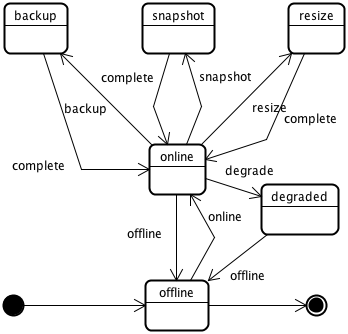
\includegraphics[scale=0.4]{figs/storage-state.png}
	\caption{State diagram for Storage}
	\label{fig:storage_state}
\end{figure}

\subsection{Linking Infrastructure Resources}
In order to create entities like virtual data centres or virtual clusters, it is necessary to allow the linking of the various infrastructure Resource types. This can be accomplished extending the core specification Link entity as the Link entity does not include enough information about specific types of infrastructure links.

\subsubsection{Linking to Network Resources}
NetworkInterface represents an L2 client device (e.g. network adapter). It can be extended using the mix-in mechanism or sub-classed to support L3/L4 capabilities such as TCP/IP etc. 

The Networkinterface Link type is assigned the http://schemas.ogf.org/occi/infrastructure\#networkinterface Category. A Networkinterface Link instance MUST use and expose this Category.

\paragraph{Attributes}
The attributes that MUST be exposed by an instance of the NetworkInterface Link type are as follows:

\begin{tabular}{lllll}
Attribute&Type&Multiplicity&Mutability&Description\\
\hline
occi.networklink.interface & String & 1 & Immutable & Identifier that relates the link to the link's device interface\\
occi.networklink.mac & String & 1 & Mutable & MAC address associated with the link's device interface\\
occi.networklink.state & String Enumeration\{ active, inactive \}& 1 & Immutable & Current status of the instance.\\
\end{tabular}

\paragraph{States}
Depicted below are the states that a NetworkInterface instance can hold.

\begin{figure}[!h]
	\centering
	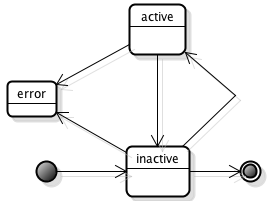
\includegraphics[scale=0.4]{figs/infra-link-state.png}
	\caption{State diagram for NetworkInterface}
	\label{fig:networklink_state}
\end{figure}

\paragraph{IPNetworkInterface Mixin}
In order to support L3/L4 capabilities (e.g. IP, TCP etc) with the NetworkInterface Link type an OCCI mixin is herewith defined.

The IPNetworkInterface mixin is assigned the http://schemas.ogf.org/occi/infrastructure/networkinterface\#ipnetworkinterface Category. An IPNetworking mixin MUST use and expose this Category.

\begin{tabular}{lllll}
Attribute&Type&Multiplicity&Mutability&Description\\
\hline
occi.networkinterface.ip & IPv4 or IPv6 Address & 1 & Mutable & Internet Protocol(IP) network address (e.g. 192.168.0.1/24, fc00::/7) of the link\\
occi.networkinterface.gateway & IPv4 or IPv6 Address & 0\ldots1 & Mutable & Internet Protocol(IP) network address (e.g. 192.168.0.1/24, fc00::/7)\\
occi.networkinterface.allocation & String Enumeration, \{dynamic, static\} & 1 & Mutable & Address mechanism: dynamic use the dynamic host configuration protocol, static uses user supplied static network configurations.\\
\end{tabular}

\subsubsection{Linking to Storage Resources}
StorageLink Link type represents a link from a Resource to a target Storage Resource.

The StorageLink Link type is assigned the  http://schemas.ogf.org/occi/infrastructure\#storagelink Category. A StorageLink Link instance MUST use and expose this Category.

\paragraph{Attributes}
The attributes that MUST be exposed by an instance of the StorageLink Link type are as follows:

\begin{tabular}{lllll}
Attribute&Type&Multiplicity&Mutability&Description\\
\hline
occi.storagelink.deviceid & String & 1 & Mutable & Device identifier as defined by the IEEE ??? standard.\\
%occi.storagelink.osdevice & String & 0\ldots1 & Mutable & Device identifier as presented to the guest OS.\\
occi.storagelink.mountpoint & String & 0\ldots1 & Mutable & Point to where the storage is mounted in the guest OS.\\
occi.storagelink.state & String Enumeration\{ active, inactive \}& 1 & Immutable & Current status of the instance.\\
\end{tabular}

\paragraph{States}
Depicted below are the states that a StorageLink instance can hold.

\begin{figure}[!h]
	\centering
	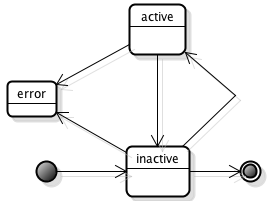
\includegraphics[scale=0.4]{figs/infra-link-state.png}
	\caption{State diagram for StorageLink}
	\label{fig:storagelink_state}
\end{figure}

\subsection{Infrastructure Templates}
There are 2 supported infrastructural template types in OCCI.

\subsubsection{OS Template}
OCCI implementers SHOULD support this, otherwise what they provision will be merely Resources without any execution environment (e.g. operating system). Of the two supported template types, this is the most basic and necessary template category that a provider SHOULD offer. The construction of it consists of a provider specific 'scheme' and a descriptive 'title' detailing the OS. The 'term' value of the template category is a provider specific identifier that corresponds to a particular virtual machine image configuration. A provider-defined OS Template Category MUST be related to the OCCI OS Template Category in order to give absolute type information. The OS Template Category is defined by the http://schemas.ogf.org/occi/infrastructure\#os\_tpl Category.

A typical example of such a category is shown below using the HTTP rendering. 

\begin{verbatim}
POST /compute
Category: compute; scheme='http://schemas.ogf.org/occi/infrastructure#'; title='Compute Instance', 
    ubuntu-9.10; scheme='http://provider.com/templates/os#'; title='Ubuntu 9.10'
Attribute: occi.compute.memory=0.5, occi.compute.cores=2
\end{verbatim}
In the example a provider has defined an OS template which offers the ability to run Ubuntu Linux upon a client's provisioned compute resource.

How a provider manages their set of OS templates will be determined by themselves and so provider-specific.

\subsubsection{Resource Template}
The Resource Template Category builds upon the concept of OS Templates. A Resource Template is a provider-defined Category that refers to a preset Resource configuration. The provider will associate a pre-determined set of Resource attributes with a particular term identifier. A provider-defined Resource Template Category MUST be related to the OCCI Resource Template Category. The Resource Template Category is defined by the http://schemas.ogf.org/occi/infrastructure\#resource\_tpl Category.

A typical example of such a Category's use is shown below using the HTTP rendering. 

\begin{verbatim}
POST /compute
Category: compute; scheme='http://schemas.ogf.org/occi/infrastructure#'; title='Compute Instance', 
    small; scheme="http://provider.com/templates/compute#"; title="Small Instance", 
    ubuntu-9.10; scheme=""; title=""
\end{verbatim}

In this example, the provider offers Compute Resources based on different sizes (small, medium, large). Each 'size' of Compute Resource corresponds to a predetermined set of OCCI attributes. In the example below a "small" Compute Resource is provisioned. Specifying "small" corresponds to a Compute Resource Attribute set of:

\begin{verbatim}
Attribute: occi.compute.cores='2', occi.compute.speed='2.4', 
    occi.compute.memory='1.0', occi.compute.arch='x86'
\end{verbatim}

How a provider manages from the administrative context their set of Resource Templates will be determined by themselves and so provider-specific.

% end infrastructure content

\section{Contributors}

Editors: Andy Edmonds, Thijs Metsch \\
Contributors: Alexander Papaspyrou, Ralf Nyr\'en, Sam Johnston

\textbf{TBD: Bunch op people missing here - create table\ldots}

\begin{verbatim}

\end{verbatim}

\section{Glossary}
\begin{tabular}{l|p{12cm}}
Term & Description \\
\hline
\hl{Action} & An OCCI base type. Represent an invocable operation on a \hl{Entity} sub-type instance or collection thereof. \\

\hl{Category} & A type in the OCCI model. The parent type of \hl{Kind}. \\

\hl{Client} & An OCCI client.\\

\hl{Collection} & A set of \hl{Entity} sub-type instances all associated to a particular \hl{Kind} or \hl{Mixin} instance. \\

\hl{Entity} & An OCCI base type. The parent type of \hl{Resource} and \hl{Link}. \\

\hl{Kind} & A type in the OCCI model. A core component of the OCCI classification system. \\

\hl{Link} & An OCCI base type. A \hl{Link} instance associate one \hl{Resource} instance with another. \\

mixin & An instance of the \hl{Mixin} type associated with a {\bf resource
 instance}. The ``mixin'' concept as used by OCCI {\em only} applies to
 instances, never to \hl{Entity} types. \\

\hl{Mixin} & A type in the OCCI model. A core component of the OCCI classification system. \\

\hl{OCCI} & Open Cloud Computing Interface \\

OCCI base type & One of \hl{Entity}, \hl{Resource}, \hl{Link} or \hl{Action}. \\

OGF & Open Grid Forum \\

\hl{Resource} & An OCCI base type. The parent type for all domain-specific resource types. \\

resource instance & An instance of a sub-type of \hl{Entity}. The OCCI
 model defines two sub-types of \hl{Entity}, the \hl{Resource} type and the
 \hl{Link} type. However, the term {\em resource instance} is defined to
 include any instance of a {\em sub-type} of \hl{Resource} or \hl{Link} as
 well. \\

Tag & A \hl{Mixin} instance with no attributes or actions defined. \\

Template & A \hl{Mixin} instance which if associated at resource instantiation
time pre-populate certain attributes. \\

type & One of the types defined by the OCCI model.  The OCCI model types are
 \hl{Category}, \hl{Kind}, \hl{Mixin}, \hl{Action}, \hl{Entity}, \hl{Resource}
 and \hl{Link}. \\

URI & Uniform Resource Identifier \\
URL & Uniform Resource Locator \\
URN & Uniform Resource Name \\
\end{tabular}


\section{Intellectual Property Statement}
The OGF takes no position regarding the validity or scope of any
intellectual property or other rights that might be claimed to pertain
to the implementation or use of the technology described in this
document or the extent to which any license under such rights might or
might not be available; neither does it represent that it has made any
effort to identify any such rights. Copies of claims of rights made
available for publication and any assurances of licenses to be made
available, or the result of an attempt made to obtain a general
license or permission for the use of such proprietary rights by
implementers or users of this specification can be obtained from the
OGF Secretariat.

The OGF invites any interested party to bring to its attention any
copyrights, patents or patent applications, or other proprietary
rights which may cover technology that may be required to practice
this recommendation. Please address the information to the OGF
Executive Director.


\section{Disclaimer}
This document and the information contained herein is provided on an
``As Is'' basis and the OGF disclaims all warranties, express or
implied, including but not limited to any warranty that the use of the
information herein will not infringe any rights or any implied
warranties of merchantability or fitness for a particular purpose.


\section{Full Copyright Notice}
Copyright \copyright ~Open Grid Forum (2009-2014). All Rights Reserved.

This document and translations of it may be copied and furnished to
others, and derivative works that comment on or otherwise explain it
or assist in its implementation may be prepared, copied, published and
distributed, in whole or in part, without restriction of any kind,
provided that the above copyright notice and this paragraph are
included on all such copies and derivative works. However, this
document itself may not be modified in any way, such as by removing
the copyright notice or references to the OGF or other organizations,
except as needed for the purpose of developing Grid Recommendations in
which case the procedures for copyrights defined in the OGF Document
process must be followed, or as required to translate it into
languages other than English.

The limited permissions granted above are perpetual and will not be
revoked by the OGF or its successors or assignees.


\section{References}

Note that only permanent documents should be cited as references. Other items, such as Web pages or working groups, should be cited inline (i.e., see the Open Grid Forum, http://www.ogf.org). References should conform to a standard such as used by IEEE/ACM, MLA, Chicago or similar. Include an author, year, title, publisher, place of publication. For online materials, also add a URL. It is acceptable to separate out ''normative references,'' as IETF documents typically do. Some sample citations: 

\end{document}
